\documentclass{article}

\usepackage{amsmath}
\usepackage{amssymb}
\usepackage{amsthm}
\usepackage{epstopdf}
\usepackage{fancyhdr}
\usepackage{fancyvrb}
\usepackage{gensymb}
\usepackage{geometry}
\usepackage{graphicx}
\usepackage{pgfplots}
\usepackage{relsize}
\usepackage{setspace}
% \usepackage{subfigure} % Deprecated package
\usepackage{subcaption}
\usepackage{tikz}
\usepackage[colorlinks,linkcolor=blue]{hyperref}

\geometry{a4paper,left=2cm,right=2cm,top=2cm,bottom=2cm}
\setlength{\parindent}{2em}
\setlength{\baselineskip}{20pt}
\linespread{1.5}
\pagestyle{fancy}
\lhead{Name: Jingyu SUN, ID: 23220003068}
\chead{}
\rhead{OOR Assignment 1}
\lfoot{}
\cfoot{}
\rfoot{\thepage}
{
    \theoremstyle{definition}
    \newtheorem{question}{Question}
    \newtheorem{solution}{Solution}
}

\begin{document}
    \title{Optimization and Operations Research Assignment 1}
    \author{Jingyu SUN}
    \maketitle
    \begin{question}
        Translate the following scenario into a linear program.\par
        A maths lecturer is visiting OUC.\par
        It is currently 9:40am and they have a class that starts at 10:10am. They would like a coffee before class, so will go from their office to the coffee shop and then to the classroom. The route they will take is shown in the picture below.\par
        For the first part of their journey they will walk slowly (shown in blue). For the second part of their journey they will walk fast (shown in purple). For the last part of their journey they will run (shown in red).\par
        The length of each part of this journey shown in the picture an indication only, the lecturer would like to figure out how long each part of the route should be.\par
        The total length of the journey is 1 km. The lecturer would like to use less than 250 kJ in energy to make this journey. Speed and energy required for slow walking, fast walking and running are shown in the table below.\par
        
        \begin{table}[htbp]
            \centering
            \begin{tabular}{c|c|c|c}
                & Slow walk & Fast walk & Run\\
                \hline
                Speed (km/hr) & 3 & 6 & 12\\
                Energy (kJ/hr) & 734 & 1304 & 3586\\
            \end{tabular}
        \end{table}

        Similar to the route shown in the picture they intend to walk (slow or fast) for most of the journey. The distance walked at a fast pace should be no more than the distance walked slowly. The distance run should be no more than half the distance walked fast.\par
        It takes 15 minutes to order and drink a coffee (during this time the lecturer stops at the coffee shop and neither walks or runs).\par
        How far should the lecturer walk slowly, walk fast and run in order to get to class as quickly as possible?\par
        (a) State the variables (including units), the objective and the constraints.\par
        (b) \textbf{MATLAB Grader.} Enter your linear program from part (a), and solve it using linprog.\par
        (c) Using the output from linprog, state the optimal solution. This should include the value of the objective and the values of the variables. Make sure you include units for all quantities.\par
        (d) How much energy does the lecturer use to make this journey?\par
        (e) Does the lecturer get to the classroom on time? How many minutes is the lecturer early (or late!) to class?\par
    \end{question}
    \begin{solution}
        (a) For this real-world problem, since the lecturer would like to figure out how long each part of the route would be, so we will define the variables as the lengths (Unit: km) for three parts, that is,
        \begin{align*}
            &x_1 := \text{the distance that the lecture slow walks}\\
            &x_2 := \text{the distance that the lecture fast walks}\\
            &x_3 := \text{the distance that the lecture runs}
        \end{align*}
        Knowing that the total length of the journey is 1km and the total energy should be less than 250kJ, we can firstly write down two constraints:
        \begin{align}
            x_1 + x_2 + x_3 = 1
        \end{align}
        \begin{align}
            \frac{x_1}{3} \times 734 + \frac{x_2}{6} \times 1304 + \frac{x_3}{12} \times 3586 \leqslant 250
        \end{align}
        Now also consider that the distances walked at different paces also have some restrictions, we have that
        \begin{align}
            x_2 \leqslant x_1
        \end{align}
        \begin{align}
            x_3 \leqslant \frac{x_2}{2}
        \end{align}
        While remember that the distances should be non-negative, we have that
        \begin{align}
            x_1 \geqslant 0, x_2 \geqslant 0, x_3 \geqslant 0
        \end{align}
        And the objective of this linear programming is to minimize the time, which is
        \begin{align*}
            \text{min} \quad z & = \frac{x_1}{3} \times 60 + \frac{x_2}{6} \times 60 + \frac{x_3}{12} \times 60 \\
            & = 20 \cdot x_1 + 10 \cdot x_2 + 5 \cdot x_3
        \end{align*}

        (b) Use the following code, we have the optimal solution and the optimal value.
        \VerbatimInput[frame=single,label=Question 1]{Question1.m}
        
        (c) The output from the linprog shows that the optimal solution for this linear program is $[0.4,0.4,0.2]^{T}$ (Unit: km) and the optimal solution is 0.2167 (Unit: hour).\par
        That means the distances for each part are 0.4km, 0.4km, 0.2km and the total time cost is 0.2167 hour (except the time stay in coffee shop).

        (d) With the distances for each part and the energy cost for each part, we have that the total energy is
        \begin{align*}
            \frac{0.4}{3} \cdot 734 + \frac{0.4}{6} \cdot 1304 + \frac{0.2}{12} \cdot 3586 \approx 244.5667 \quad \text{(Unit: kJ)}
        \end{align*}

        (e) Since the lecturer spend 0.2167 hour in the whole path and 15 minutes for staying in the coffee shop, the total time (Unit: minutes) the lecturer spend is
        \begin{align*}
            0.2167 \cdot 60 + 15 = 18 \quad \text{(Unit: minutes)}
        \end{align*}
    \end{solution}
    \begin{question}
        Consider the following linear program
        \begin{align}
            \text{max} \quad z = 2x + 2y ,
            \label{objective2}
        \end{align}
        subject to
        \begin{align*}
            -3x - y \leqslant -3&\\
            -2x + y \leqslant 3&\\
            y \leqslant 5&\\
            3x + y \leqslant 14&\\
            2x - y \leqslant 6&
        \end{align*}
        with $x, y \geqslant 0$.\par
        (a) Draw the feasible region. Do this either by hand or with MATLAB (or similar). Your drawing should include:
        \begin{itemize}
            \item the edges of the feasible region
            \item the vertices of the feasible region
        \end{itemize}
        \textbf{Hint}: start by drawing one line for each constraint to show the edges of the feasible region.\par
        To get you started, here is a line representing the first constraint:\par
        (b) Consider the region from part (a). State the feasible vertices. How many are there?\par
        (c) Calculate the objective at each feasible vertex. What is the optimal solution?\par
        (d) You should find that \textbf{two pairs} of vertices have the same value of the objective function. Explain what is happening here with reference to both the objective function and the shape of feasible region.\par
        Finally, state \textbf{with some explanation} a different objective function of the form $z = ax +by$ with the following properties:\par
        \begin{itemize}
            \item there are two pairs of vertices with the same value of the objective.
            \item there is a unique maximum to the linear program.
            \item the coefficients of the objective are not equal, that is $a\ne b$.
        \end{itemize}\par
        (e) \textbf{MATLAB Grader.} Check your answer using linprog.
    \end{question}
    \begin{solution}
        (a) The edge of the feasible region is shown in figure \ref{figure1}, and by finding the public region, the feasible region is shown in figure \ref{figure2}.\par
        \begin{figure}[htbp]
            \begin{subfigure}[b]{0.45\textwidth}
                \centering
                \begin{tikzpicture}[scale=0.7]
                    \draw[->, thick] (0,0) -- (6,0) node[right] {$x$};
                    \draw[-, thick] (-2,0) -- (0,0);
                    \draw[->, thick] (0,0) -- (0,9) node[above] {$y$};
                    \draw[-, thick] (0,-5) -- (0,0);
                    \draw[red] (-1,6) -- (2,-3);
                    \draw[red] (-1,0) -- (5,0);
                    \draw[red] (1,-4) -- (6,6);
                    \draw[red] (5,-1) -- (2,8);
                    \draw[red] (6,5) -- (-1,5);
                    \draw[red] (3,9) -- (-1,1);
                \end{tikzpicture}
                \caption{Feasible Region Constraints}
                \label{figure1}
            \end{subfigure}
            \hfill
            \begin{subfigure}[b]{0.45\textwidth}
                \centering
                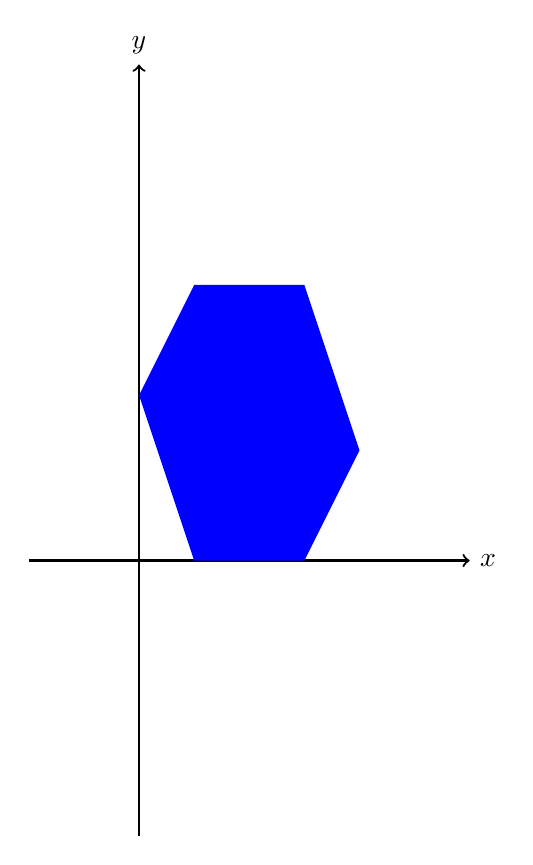
\begin{tikzpicture}[scale=0.7]
                    \draw[->, thick] (0,0) -- (6,0) node[right] {$x$};
                    \draw[-, thick] (-2,0) -- (0,0);
                    \draw[->, thick] (0,0) -- (0,9) node[above] {$y$};
                    \draw[-, thick] (0,-5) -- (0,0);
                    \fill[blue] (0,3) -- (1,0) -- (3,0) -- (4,2) -- (3,5) -- (1,5) -- (0,3) -- cycle;
                \end{tikzpicture}
                \caption{Feasible Region Shape}
                \label{figure2}
            \end{subfigure}
            \caption{Feasible Region}
        \end{figure}

        (b) By solving the constraints and the above feasible region, we have the following feasible vertices:\par
        $$(0,3), (1,0), (3,0), (4,2), (3,5), (1,5)$$
        
        (c) Now having five feasible vertices and the objective funtion $ z = 2x + 2y $, we will have each optimal solution:\par
        $$ z(0,3) = 6, z(1,0) = 2, z(3,0) = 6, z(4,2) = 12, z(3,5) = 16, z(1,5) = 12 $$

        (d) From (c), we have that:
        \begin{itemize}
            \item $(4,2)$ and $(1,5)$ both have $z=12$.
            \item $(0,3)$ and $(3,0)$ both have $z=6$.
        \end{itemize}

        The reason that this happens is that the coefficients of the objective funtion (\ref{objective2}) have $a = 2$ and $b = 2$, so in geometry languages, the objective funtion on the feasible region is parallel to the straight line that links these two pairs of vertices, like what figure \ref{figure1} shows. This makes the objective function have the same value at these paired vertices.\par 
        Now, consider the mentioned properties, a good objective function would be $z = x$. And we will check each properties:\par
        \begin{itemize}
            \item There are two pairs of vertices with the same value of the objective: $(1,5)$ and $(1,0)$ both have $z=1$, $(3,5)$ and $(3,0)$ both have $z=3$.
            \item There is a unique maximum to the linear program: the unique maximum will occur at $(4,2)$ because $(0,3)$ has value $z=0$ and above shows other 4 points' value.
            \item The coefficients of the objective are not equal, which we have $a=1, b=0$.
        \end{itemize}

        (e) Using the following code, we can check the answer using linprog.
        \VerbatimInput[frame=single,label=Question 2]{Question2.m}

        And it turns out the optimal solution for this program is $[3,5]^{T}$ and the optimal value is 16.\par
    \end{solution}
\end{document}